% Created 2023-03-18 Σαβ 15:44
% Intended LaTeX compiler: pdflatex
\documentclass[breaklines=true]{report}
\usepackage[utf8]{inputenc}
\usepackage[T1]{fontenc}
\usepackage{graphicx}
\usepackage{longtable}
\usepackage{wrapfig}
\usepackage{rotating}
\usepackage[normalem]{ulem}
\usepackage{amsmath}
\usepackage{amssymb}
\usepackage{capt-of}
\usepackage{hyperref}
\usepackage{minted}
\usepackage[margin=2cm]{geometry}
\usepackage{setspace}
\usepackage[utf8]{inputenc}
\usepackage[LGR]{fontenc}
\usepackage[T1]{fontenc}
\usepackage[english, greek, ]{babel}
\newcommand{\en}[1]{\foreignlanguage{english}{#1}}
\usepackage{minted}
\hypersetup{colorlinks=true, linkcolor=black}
\usepackage{bookmark}
\usepackage{fancyhdr}
\usepackage{lipsum}% just to generate text for the example
\pagestyle{fancy}
\fancyhf{}
\fancyhead[L]{\rightmark}
\fancyhead[R]{\leftmark}
\renewcommand{\headrulewidth}{0.4pt}
\author{Νικόλας Τοροσιάν Νίκος Παπαδάκης}
\date{\today}
\title{Φίλτρα συχνοτήτων και απομόνωση Η/Μ θορύβου}
\hypersetup{
 pdfauthor={Νικόλας Τοροσιάν Νίκος Παπαδάκης},
 pdftitle={Φίλτρα συχνοτήτων και απομόνωση Η/Μ θορύβου},
 pdfkeywords={},
 pdfsubject={},
 pdfcreator={Emacs 28.2 (Org mode 9.6.1)}, 
 pdflang={Gr}}
\begin{document}

\maketitle
\tableofcontents

\part{Εισαγωγή}
\label{sec:org32eefcc}
Σε πολλές περιπτώσεις η ανάγκη της επεξεργασίας σημάτων, όπως στις
τηλεπικοινωνίες μετά ή/και πριν την μετάδοση από τον πομπό προς τον
δέκτη, και η εκλογή πληροφοριών από αυτό έθεσαν από νωρίς το πρόβλημα
των παρεμβολών του περιβάλλοντος στις ηλεκτρονικές συσκευές και την
ανάγκη απομόνωσης του φάσματος των συχνοτήτων που χρησιμοποιούνται για
κάθε λειτουργία.

Η απομόνωση αυτή μπορεί να επιτευχθεί είτε μέσω συμβατικών φίλτρων,
δηλαδή αντιστάσεις και πυκνωτές κατάλληλα τοποθετημένους στο κύκλωμα που
συλλέγει την τάση (\textbf{ρεύμα μέτρησης}), είτε με την χρήση μεθόδων ψηφιακής
επεξεργασίας σημάτων ( \(\en{DSP}\) ).
Στις μέρες μας προτιμάται ο 2ος τρόπος λόγω
της ραγδαίας εξέλιξης των Η/Υ με αποτέλεσμα να επιφέρει μεγαλύτερο
κόστος η εγκατάσταση αναλογικών φίλτρων σε κάθε θέση που απαιτείται.

Οι μέθοδοι αλλά και η πληθώρα συστημάτων λήψης και ανάλυσης σημάτων τις
τελευταίες δεκαετίες έχουν, αφενός εξελιχθεί ως προς την υπολογιστική
ισχύ με γρηγορότερους επεξεργαστές και αλγόριθμους, αφετέρου δίνουν
πλέον την δυνατότητα διαχείρισης των πληροφοριών απομακρυσμένα με
αποτέλεσμα την ευρύτερη εγκαθίδρυση των ψηφιακών μέσων επεξεργασίας
σημάτων. Στις μέρες μας η ανάγκη διαχείρισης ολοένα και μεγαλύτερα
αρχεία δεδομένων με καλύτερη ακρίβεια οδήγησε την επιστημονική κοινότητα
στην χρήση της μεθόδου \textbf{μετα-επεξεργασίας} (\(\en{post-processing}\)). Βασικό όφελος
ήταν η δυνατότητα επαναληψιμότητας του πειράματος και σύγκρισης των
αποτελεσμάτων σε όλο τον κόσμο, ουσιαστική αρχή της πειραματικής
διαδικασίας. Έτσι με την χρήση προγραμματισμού δίνεται πλέον η
δυνατότητα στον ερευνητή, να δημιουργεί ένα περιβάλλον προσομοίωσης και
να δοκιμάζει διάφορες λύσεις χωρίς να επισκεφτεί την πειραματική διάταξη
σε πολλές περιπτώσεις μετά την καταγραφή των μετρήσεων.

Στην παρούσα εργασία θα πραγματευτούμε την απομείωση συγκεκριμένων
συχνοτήτων με την χρήση Ψηφιακής Ανάλυσης Σημάτων και φίλτρων, διαφόρων
κατηγοριών. Στο πλαίσιο αυτό θα παρουσιαστεί, μια μελέτη που
πραγματοποιήθηκε σε συνεργασία με το εργαστήριο Αιολικής Ενέργειας του
τμήματος Μηχανολόγων Μηχανικών στο Ελληνικό Μεσογειακό Πανεπιστήμιο με
θέμα την απόρριψη θορύβου από αισθητήριο όργανο για την μέτρηση της
ταχύτητας ανέμου σε περιβάλλον με ενισχυμένες παρεμβολές. Η
ιδιαιτερότητα που παρουσιάστηκε στην εγκατάσταση ήταν παρεμβολές από
ηλεκτρικό μετασχηματιστή, που όμως ήταν αδύνατο να
αφαιρεθεί, και ταυτόχρονα ο σχεδιασμός όπως και η τοποθέτηση ενός
αναλογικού φίλτρου θα ενέτασαν μεγάλο κόστος και περιπλοκότητα. Θα
αναλυθούν οι δομές σημάτων που επεξεργάστηκαν καθώς και οι τύποι των
φίλτρων που χρησίμευσαν στην απομόνωση των ζητούμενων σημάτων. Επίσης θα
υπάρξει παράθεση των θετικών και αρνητικών που παρατηρήθηκαν κατά την
διάρκεια εκτέλεσης της επεξεργασίας και καταγραφής των δεδομένων (τύποι
αρχείων δεδομένων). Τέλος θα ήθελα να ευχαριστήσω τον καθηγητή μου κ.
Νίκο Παπαδάκη για την καθοδήγησή του και την υπομονή που έδειξε για τις
λιγοστές γνώσεις μου στον προγραμματισμό.

\noindent\rule{\textwidth}{0.5pt}
\part{Ιστορική αναδρομή}
\label{sec:org588e4f0}
Από την εποχή της ανακάλυψης του Απειροστικού λογισμού \((\en{calculus})\)
τον 17ο αιώνα, οι επιστήμονες προσπαθούν να εξηγήσουν τα φυσικά
φαινόμενα με μαθηματικά μοντέλα χρησιμοποιώντας εξισώσεις
συνεχών μεταβλητών και διαφορικές εξισώσεις. Χρησιμοποιήθηκαν
τεχνικές αριθμητικής επίλυσης όταν οι αναλυτικές λύσεις δεν
ήταν εφικτό να καθοριστούν. Αργότερα μαθηματικοί του 18ου αιώνα
όπως οι Ευλερ, Μπερνούλι και Λαγκραντζ κατασκεύασαν μεθόδους
για αριθμητική ολοκλήρωση και την εισαγωγή εξισώσεων συνεχών
μεταβλητών. Μια ιστορική μελέτη από τους \(\en{Heideman, Johnson}\) και
\(\en{Burrus}\) (1984) έδειξε ότι ο \(\en{Gauss}\) είχε ανακαλύψει την βασική
αρχή του γρήγορου μετασχηματισμού \(\en{Fourier}\) ήδη από το 1805, πριν
την δημοσίευση της διατριβής του \ldots{}. πάνω στην απεικόνιση
αρμονικών σειρών εξισώσεων.
Στις αρχές του 1950, η ανάλυση σημάτων γινόταν κυρίως με
αναλογικά συστήματα κατασκευασμένα από ηλεκτρονικά κυκλώματα
ακόμα και με μηχανικές συσκευές. Ενώ οι Η/Υ είχαν κάνει την
είσοδό τους ήδη σε επιχειρήσεις και επιστημονικά εργαστήρια
ήταν ακόμα ακριβοί με περιορισμένες δυνατότητες. Περίπου εκείνη
την εποχή ξεκίνησε η ανάγκη για πιο εξειδικευμένες μεθόδους
στην ανάλυση σημάτων και στράφηκε η προσοχή στην ανάλυση
διακριτού χρόνου σημάτων. Μια από τις πρώτες εφαρμογές των Η/Υ
ήταν η καταγραφή σεισμικών δονήσεων σε πλατφόρμες εξόρυξης
πετρελαίου, που καταγράφονταν σε μαγνητική ταινία για να επεξεργαστούν
αργότερα. Η διαδικασία αυτή δεν μπορούσε να γίνει σε
πραγματικό χρόνο, καθώς μπορεί να χρειαζόντουσαν κάποια
λεπτά ακόμα και ώρες για την επεξεργασία μερικών δευτερολέπτων
από τις μαγνητικές ταινίες.
    Την ίδια εποχή για όσους είχαν την δυνατότητα να χρησιμοποιήσουν
ψηφιακούς υπολογιστές, ήταν εύκολο να δημιουργήσουν ένα περιβάλλον
προσομοίωσης για να μελετήσουν νέους αλγόριθμους και μεθόδους
ανάλυσης σημάτων πριν χρησιμοποιήσουν πόρους και μηχανικούς για την
κατασκευή της αναλογικής συσκευής που τελικά θα εκτελούσε την
επιθυμητή εργασία. Παραδείγματα τέτοιων προσομοιώσεων ήταν εκείνες
που πραγματοποιήθηκαν στο Εργαστήριο Λίνκολν και στα Εργαστήρια Μπελλ
όπου προσομοιώθηκε ένας κωδικοποιητής φωνής \(\en{vocoder}\). Στην κατασκευή
ενός αναλογικού καναλιού κωδικοποιητής φωνής, τα χαρακτηριστικά του
φίλτρου επηρεάζουν την ποιότητα της φωνής σε βαθμό που ήταν δύσκολο να
διακριθούν αντικειμενικά. Μέσω προγραμματισμένων προσομοιώσεων
κατάφεραν την ρύθμιση των χαρακτηριστικών, ώστε να καθορίσουν το
αποτέλεσμα της αναλογικής συσκευής πριν την κατασκευή της.
    Εδώ αξίζει να σημειωθεί ότι ενώ η χρήση των Η/Υ βοήθησε στην πειραματική
διαδικασία, μπορούσε μόνο να \emph{προσομοιώσει ή προσεγγίσει} το αναλογικό
σύστημα ανάλυσης σημάτων.

Καθώς τα σήματα ξεκίνησαν να επεξεργάζονται σε ψηφιακούς υπολογιστές, οι
ερευνητές αναγκάστηκαν πολύ γρήγορα να χρησιμοποιούν ολοένα και πιο περίπλοκους
αλγόριθμους επεξεργασίας σημάτων. Πολλοί από τους αλγόριθμους
εξελίχθηκαν λόγω της ευελιξίας που παρείχε το προγραμματιστικό περιβάλλον
σε αντίθεση με την μόνιμη αναλογική κατασκευή, όπου περιορίζεται η δυνατότητα
πειραματισμού. Έτσι η συνεχής εξέλιξη και ευελιξία της ψηφιακής
επεξεργασίας σημάτων έδωσε το έναυσμα για την ολική ψηφιοποίηση των συσκευών
και μεθόδων της επεξεργασίας και διάδοσης σημάτων στην πλειοψηφία των
εγκαταστάσεων. Εκείνη την περίοδο ξεκίνησε ενεργά η δημιουργία ψηφιακών
κωδικοποιητών φωνής, ψηφιακών αναλυτών φάσματος κ.α. συσκευών αμιγώς ψηφιακής
επεξεργασίας σήματος, με την ελπίδα ότι τελικά τέτοια συστήματα θα
αποκτούσαν πρακτικές εφαρμογές.

Μία νέα σκοπιά προς την επεξεργασία σημάτων διακριτού χρόνου επιταχύνθηκε
με την δημοσίευση από τους \(\en{Cooley\ and\ Tukey}\) (1965) ενός αποδοτικού αλγόριθμου
για τον υπολογισμό του μετασχηματισμού \(\en{Fourier}\). Η κλάση αυτή θα γίνει
αργότερα γνωστή ως Ταχύς Μετασχηματισμός \(\en{Fourier (F.F.T.\ Fast\ Fourier\ Transform)}\).
Ο \(\en{F.F.T.}\) ήταν αρκετά σημαντικός για πολλούς λόγους. Βασικό
πρόβλημα των αλγόριθμων της εποχής ήταν ότι απαιτούσαν χρόνους
επεξεργασίας πολύ μεγαλύτερους από τον πραγματικό χρόνο του
καταγεγραμμένου σήματος. Αυτό συνέβαινε γιατί στις περισσότερες
περιπτώσεις απαιτείται η χρήση ανάλυσης φάσματος του σήματος και μέχρι
τότε δεν υπήρχε κάποιος αποδοτικός αλγόριθμος. Ο ταχύς μετασχηματισμός
προσέφερε την δυνατότητα στους ερευνητές να πειραματίζονται σε
πραγματικούς χρόνους με την εγκατάσταση, καθώς μείωσε δραστικά τον χρόνο
επεξεργασίας κατά πολλές τάξεις μεγέθους. Επιπρόσθετα πολλοί αλγόριθμοι
που δεν είχαν καμία πρακτική εφαρμογή, λόγω του χρόνου επεξεργασίας,
ξεκίνησαν να έχουν πρακτικές εφαρμογές στην βιομηχανία και αργότερα στα
προϊόντα για τον γενικό πληθυσμό.

Άλλη μια σημαντική ιδιότητα του \(\en{F.F.T.}\) που βοήθησε στον σχεδιασμό καλύτερων
συσκευών ήταν ότι προγραμματίστηκε με βάση τα σήματα διακριτού χρόνου.
Δηλαδή εμπεριείχε τις απαιτούμενες ιδιότητες και μαθηματικά ώστε να
διαχειρίζεται ψηφιοποιημένα σήματα -διακριτού χρόνου- και να μην
\emph{προσομοιώνει} μια αναλογική συμπεριφορά ενός σήματος ή συστήματος.
Έτσι η δυνατότητα σχεδιασμού συστημάτων που προβλεπόταν η ακριβής
συμπεριφορά του βοήθησε στην εξέλιξη της επεξεργασίας σημάτων
διακριτού χρόνου χωρίς την ανάγκη συσχέτισης των αποτελεσμάτων
με ένα σύστημα συνεχούς χρόνου (αναλογικού συστήματος). Έτσι η ένταξη
των διακριτών σημάτων ως ξεχωριστή μέθοδος επεξεργασίας προσέφερε στην
ανάπτυξη τεχνολογίας μειώνοντας, εκτός από τους απαιτούμενους χρόνους,
το κόστος και τον όγκο των εγκαταστάσεων για την επίτευξη του στόχου.

Παράλληλα η επινόηση και εφεύρεση των μικρο-ελεγκτών στον τομέα της
μικροηλεκτρονικής επέφερε περαιτέρω μείωση του κόστους. Ενώ οι
πρώτες συσκευές μικρο-ελεγκτών δεν παρείχαν τις απαιτούμενες δυνατότητες
για την ολοκλήρωση των συστημάτων επεξεργασίας διακριτών σημάτων, από
τις αρχές της δεκαετίας του '80 η ταχύτητα τους αυξάνεται εκθετικά.
Επιπρόσθετα η αρχιτεκτονική και τεχνολογία των ολοκληρωμένων κυκλωμάτων
(\(\en{I.C.\ Intergated\ Circuit}\)) αναπτύχθηκε προς την κατεύθυνση για την κατασκευή
ολοένα και ταχύτερων υπολογιστών για την διαχείριση ακέραιων και δεκαδικών
αριθμών. Έτσι σήμερα η ανάλυση σημάτων, η καταγραφή όπως και η μετάδοσή τους
γίνεται πολλές φορές εξ' ολοκλήρου από ψηφιακά συστήματα.

\noindent\rule{\textwidth}{0.5pt}
\part{Σήματα}
\label{sec:org0ac7f34}
\chapter{Εισαγωγή}
\label{sec:orge37b226}
Ο όρος σήμα \(\en{(signal)}\) δίνεται σε κάτι που εμπεριέχει πληροφορία. Γενικά
τα σήματα χρησιμοποιούνται στην κωδικοποίηση και εξαγωγή πληροφοριών για
την κατάσταση ή/και την συμπεριφορά ενός φυσικού συστήματος. Συχνά
συνδυάζοντας διαφορετικά σήματα υπάρχει η δυνατότητα επικοινωνίας μεταξύ
ανθρώπων αλλά και με μηχανήματα. Άν και αναπαριστούμε τα σήματα με διάφορες
μορφές η πληροφορία που μεταδίδουν, εμπεριέχεται με την μορφή μοτίβων. Η
μαθηματική αναπαράσταση παρέχεται μέσω συνάρτησης μίας ή περισσότερων
ανεξάρτητων μεταβλητών. Ένα παράδειγμα είναι η ανεξάρτητη μεταβλητή της
εξίσωσης που περιγράφει μία ψηφιακή εικόνα, όπου θα αποτελείται από δύο
χωρικές μεταβλητές σε συνάρτηση της φωτεινότητας. Αντίθετα ένα αρχείο ήχου
θα ορίζεται σε συνάρτηση με τον χρόνο. Εδώ καταχρηστικά όταν θα αναφερόμαστε
σε κάποιο σήμα θα χρησιμοποιούμε την 2η περίπτωση, δηλαδή ως προς τον χρόνο.

Η ανεξάρτητη μεταβλητή του χρόνου σε ένα σήμα μπορεί να είναι συνεχής ή
διακριτή ως προς το διάστημα που ορίζεται. Τα σήματα συνεχούς χρόνου
ορίζονται για κάθε τιμή τους στο διάστημα και επομένως αναπαριστώνται
με μία ανεξάρτητη συνεχή μεταβλητή. Στην παραπάνω περίπτωση αναφερόμαστε
σε αυτά ως \textbf{αναλογικά σήματα}. Ως \textbf{σήματα διακριτού χρόνου} ονομάζουμε όσα η
ανεξάρτητη μεταβλητή του χρόνου μας παρέχει πληροφορία για συγκεκριμένα
διαστήματα ή αλλιώς χρονικές στιγμές. Εδώ η αναπαράσταση του χρόνου γίνεται
με την χρήση ακολουθίας αριθμών, συνήθως ανά συγκεκριμένο διάστημα π.χ.
κάθε 0,1 δευτερόλεπτα. Εκτός του χρόνου την ίδια κατηγοριοποίηση συναντούμε
και στην αναπαράσταση της ισχύος ενός σήματος \((amplitute)\). \textbf{Ψηφιακά σήματα}
ονομάζονται όσα έχουν διακριτές τιμές ισχύος και χρόνου.

Τα συστήματα ανάλυσης σημάτων κατηγοριοποιούνται ανάλογα. Συστήματα συνεχούς
χρόνου ονομάζονται εκείνα που τα σήματα εισόδου και εξόδου είναι αναλογικά.
Αντίστοιχα συστήματα διακριτού χρόνου ονομάζονται όσα δαχειρίζονται σήματα
διακριτού χρόνου. Ψηφιακά συστήματα ονομάζονται όσα λαμβάνουν σε είσοδο και
έξοδο ψηφιακά σήματα. Επομένως στην ψηφιακή ανάλυση σημάτων
\(\en{(Digital\ signal\ processing)}\) επεξεργάζονται σήματα που εκφράζονται
με ακολουθίες για τον χρόνο και την ισχύ τους.

Σήματα διακριτού χρόνου προκύπτουν καταγράφοντας ένα συνεχές σήμα ή από
διεργασίες που εκτελούνται σε διακριτές τιμές του χρόνου. Ανεξαρτήτου
προέλευσης του σήματος, τα συστήματα επεξεργασίας σημάτων διακριτού χρόνου
παρέχουν πολλές δυνατότητες ελκύοντας το ενδιαφέρον τις τελευταίες
δεκαετίες. Έχουν δυνατότητες προσομοίωσης αναλογικών συστημάτων με
περισσότερη ευελιξία και παρέχουν την δυνατότητα ανακάλυψης τυχών μεταβολών
στα σήματα που δεν είναι δυνατόν να γίνουν αντιληπτά από ένα αναλογικό
σύστημα επεξεργασίας. Επιπρόσθετα η συνεχής ανάπτυξη ψηφιακών συσκευών
όπως είναι οι υπολογιστές γενικής χρήσης και οι μικρο-ελεγκτές προτιμάται
η αναπαράσταση των σημάτων σε διακριτά πεδία χρόνου αν όχι σε ψηφιακή μορφή.

Παρακάτω στο κεφάλαιο θα αναφερθούμε σε βασικές έννοιες που διέπουν τα σήματα
διακριτού χρόνου και συστήματα ανάλυσης αυτών για μονοδιάστατα σήματα.
Πρακτικά υπάρχει η δυνατότητα να διαχειριστούμε τα σήματα αυτά ως αναλογικά
και με σωστή χρήση συγκεκριμένων κριτηρίων μπορούμε να εξάγουμε τα σωστά
αποτελέσματα. Τέτοιου τύπου συστήματα καθόρισαν τις βασικές αρχές των
καταγραφικών συσκευών δεδομένων. Όμως πολλά συστήματα διακριτού χρόνου
δεν ορίζονται ως προσομοιώσεις αναλογικών συστημάτων καθώς και πολλές
ακολουθίες δεν προκύπτουν καταγράφοντας ένα αναλογικό σήμα. Για τους
παραπάνω λόγους αντί να εφαρμοστούν τα αποτελέσματα από την θεωρία που
αναφέρεται στα συνεχή σήματα-συστήματα, θα εκβάλλονται παράλληλα συμπεράσματα
ξεκινώντας από τα χαρακτηριστικά που διέπουν το σήμα και θέτοντας το
ανάλογο πλαίσιο επεξεργασίας. Εδώ ασχοληθήκαμε μόνο με ψηφιακά σήματα
καθώς η καταγραφή των σημάτων έγινε με Η/Υ μέσω προγράμματος \(\en{(Lab-View)}\).

\chapter{Συνεχούς χρόνου}
\label{sec:orgd033136}
Στην εισαγωγή αναφερθήκαμε στον γενικό ορισμό των σημάτων και τις διαφορές
που τα κατηγοριοποιούν σε αρχικό βαθμό. Επειδή ο στόχος της παρούσας εργασίας
ήταν η απόρριψη θορύβου δεν θα γίνει η πρέπουσα ανάλυση στην θεωρία των σημάτων,
αντιθέτως θα παρατεθούν οι βασικές αρχές και έννοιες ώστε να υπάρχει το υπόβαθρο
για τα επόμενα κεφάλαια. Σήμα συνεχούς χρόνου ορίζουμε ως την εξίσωση που
περιγράφει την εξέλιξη μιας περιοδικής κυματομορφής στο χρόνο. Πιο συγκεκριμένα
αν υποθέσουμε πως ο χρόνος διάρκειας του σήματος είναι \(t\) τότε η κυματομορφή στο
πεδίο του χρόνου θα εκφράζεται ως συνάρτηση αυτού \(s(t)\).

Μπορεί λοιπόν να παρασταθεί από μία ανεξάρτητη μεταβλητή και ορίζεται για κάθε
τιμή της. Με παρόμοιο τρόπο ορίζονται και τα διακριτά σήματα συνεχούς χρόνου.
Η διαφορά είναι πως αντί να μπορούμε να ταυτίσουμε κάθε χρονική στιγμή με το
αντίστοιχο \(s(t)\). Σήμα συνεχούς χρόνου ονομάζεται ένα σήμα \(y(t)\), το οποίο ορίζεται
για κάθε τιμή του \(t\) σε κάποιο διάστημα χρόνου \([\alpha,\beta]\). Συνήθως τα συναντούμε
στην μορφή συνεχούς ρεύματος σε μετρητικές και άλλες συσκευές σε εξόδους
για την ένδειξη κάποιας τιμής ή απεικόνιση σε παλμογράφο. Τα σήματα
συνεχούς χρόνου χωρίζονται σε αναλογικά και διακριτά σήματα συνεχούς
χρόνου.

Αναλογικά σήματα ονομάζονται εκείνα που η ανεξάρτητη μεταβλητή του
χρόνου \(t\) και η μεταβλητή του πλάτους (εξαρτημένη μεταβλητή ως προς τον
χρόνο) λαμβάνουν συνεχής και πραγματικές τιμές, π.χ. \(s(t) = 12 * t\).
Διακριτά σήματα συνεχούς χρόνου ονομάζονται όσα ή εξαρτημένη τιμή
(πλάτος) παίρνει διακριτές τιμές, π.χ.
\begin{equation}
\begin{align}
s(t) =  A * t \\
A &= [0, … ,n],\ t \in [a,b] n \in \mathbb{Z} \\
\end{align}
\end{equation}

Στην πληθώρα των συσκευών επεξεργασίας και καταγραφής σημάτων η χρήση
των αναλογικών σημάτων έχει σχεδόν εκλείψει. Σημαντικό μειονέκτημα
ανάμεσα σε άλλα είναι και ο υπέρογκος χώρος αποθήκευσης που απαιτείται
για την αποθήκευση του. Παρακάτω θα αναφερθούμε στα \textbf{ψηφιακά} σήματα που
έλυσαν πολλά από τα προβλήματα των αναλογικών σημάτων, προσθέτοντας μια
σειρά από "πονοκεφάλους" αρχικά στην επιστημονική κοινότητα. Τα
πλεονεκτήματα ήταν πολλά και τελικά επικράτησαν. Παρακάτω θα παρατεθούν
κάποιες βασικές έννοιες και αρχές που τα διέπουν.

\noindent\rule{\textwidth}{0.5pt}
\chapter{Διακριτού χρόνου}
\label{sec:orgcc1a3ba}
Σήμα διακριτού χρόνου ονομάζεται μια ακολουθία αριθμών καταγεγραμμένες
ανά συγκεκριμένο χρονικό διάστημα, π.χ. κάθε 0,01 δευτερόλεπτο. Το
διάστημα αυτό ορίζει την ταχύτητα καταγραφής του σήματος από την
εκάστοτε συσκευή, όμως εμείς αναφερόμαστε σε αυτό το χρόνο μέσω της
συχνότητας καταγραφής ή αλλιώς \(\en{sampling\ frequency}\). Η συχνότητα αυτή
ορίζεται ως το πηλίκο ενός δευτερολέπτου ως προς το χρονικό διάστημα
καταγραφής, δηλαδή από το παραπάνω παράδειγμα θα είχαμε μια συχνότητα
καταγραφής 1/0.01 \([Hz]\).
\begin{equation}
fs = \frac{1}{0,01} [Hz]
\end{equation}
Σημαντικό είναι να αναφερθεί ότι υπάρχει ένα όριο το οποίο πρέπει να
τηρείται ώστε η επαναδημιουργία του σήματος να απεικονίζει όσο το
δυνατόν πιο πολύ στο συνεχές σήμα που καταγράφηκε στην αρχή. Θα
αναφερθούμε αργότερα στο εν λόγω θεώρημα του φυσικού \(\en{Niquist}\).
\section{Μοναδιαίο διακριτό σήμα}
\label{sec:orgd228661}
Μοναδιαίο ονομάζεται το σήμα που αποτελείται από έναν κρουστικού
χαρακτήρα παλμού και έχει μηδενική ισχύ πρίν και μετά την εμφάνισή
του. Αν υποθέσουμε μια συνάρτηση \(y(t)\) ,
\begin{equation}
\begin{align}
y(t) = [..., 0, 1, 0, ...]
\end{align}
\end{equation}
θα είναι η έξοδος του σήματος αυτού.

Μια άλλη βασική υποκατηγορία αποτελεί η μοναδιαία ακολουθία βήματος.
Εδώ σε αντίθεση με παραπάνω, η τιμή της εξόδου αλλάζει από μηδέν σε ένα
μόλις η εξαρτημένη μεταβλητή \en{t} λάβει κάποια οριακή τιμή.
Χρησιμοποιώντας το ανωτέρω παράδειγμα θα έχουμε ότι:
\begin{equation}
\begin{align}
y(t) = [..., 0, 1, 1, 1, ...]
\end{align}
\end{equation}
\section{Τυχαίο σήμα}
\label{sec:org0f8cfb4}
Τα τυχαία σήματα αποτελούν μία ειδική υποκατηγορία που χρησιμοποιείται
ευρέως στην ανάλυση ψηφιακών σημάτων. Αναπτύχθηκαν για να καλύψουν την
ανάγκη επιβεβαίωσης των συσκευών επεξεργασίας κυματομορφών. Με την
πάροδο του χρόνου τις συναντάμε σε διάφορες συσκευές τηλεπικοινωνίας
και σχεδόν σε όλες τις συσκευές παραγωγής ήχου (\en{synthesizers}).
Αξίζει να σημειωθεί για λόγους πληρότητας ότι τα εν' λόγω σήματα
βασίζονται σε στατιστικά μοντέλα που απορρέουν από στατιστικές κατανομές.
Ο "λευκός" γκαουσιανός θόρυβος (\en{white gaussian noise}) ακολουθεί
την λεγόμενη κανονική κατανομή πιθανοτήτων του \en{Gauss}. Στην παρούσα
εργασία ένα αντίστοιχο σήμα χρησιμοποιήθηκε για την επιβεβαίωση των
φίλτρων πριν την εφαρμογή στο σετ δεδομένων. Δεν θα γίνει περαιτέρω
ανάλυση γιατί κρίθηκε πως οι παρεμβολές στον αισθητήρα της εγκατάστασης
προερχόταν από εξωτερικά Η/Μ πεδία.
\section{Διακριτά σήματα και ακολουθίες}
\label{sec:org109caec}
Για τον ορισμό του διακριτού σήματος αρκεί να υποθέσουμε μία μαθηματική
ακολουθία αριθμών \(x\), όπου το νιοστό στοιχείο της θα γραφόταν ως \(x[n]\).
Ορθότερα μπορούμε να γράψουμε την εξής έκφραση:
\begin{equation}
\begin{align}
n \in \mathbb{Z} \\
x &= {x[n]},\  -\infty < n < \infty \\
\end{align}
\end{equation}
όπου Ζ είναι σαφώς το σύνολο των ακέραιων αριθμών και \(x[n]\) το κάθε στοιχείο
της ακολουθίας. Ο συγκεκριμένος τύπος σήματος παράγεται συνήθως από την
καταγραφή αναλογικού σήματος και επομένως η παραπάνω σχέση μετασχηματίζεται
για αναλογικό σήμα της μορφής \(x_{a}(t)\) για χρονική στιγμή ίση με \(nT\) το νιοστό
στοιχείο της ακολουθίας εξόδου από την καταγραφή θα είναι της μορφής:
\begin{equation}
\begin{align}
x[n] = x_{a} nT,\ -\infty < n < \infty \\
\end{align}
\end{equation}

Η ποσότητα \(T\) ορίζει την περίοδο καταγραφής που παρέχει την συχνότητα
καταγραφής διαιρώντας με την μονάδα. Αν και τα διακριτά σήματα δεν
προέρχονται πάντα από καταγραφή αναλογικών σημάτων ο ορισμός του αριθμού
των στοιχείων της ακολουθίας \(n\) μπορεί να λάβει μόνο ακέραιες τιμές. Επίσης
γράφοντας μόνο το "τελευταίο" ψηφίο μέσα στην αγκύλη αναφερόμαστε σε όλα
τα στοιχεία της ακολουθίας για συντομία και όχι στο τελευταίο στοιχείο
αυτής.
\section{Διαχείριση και βασικές τεχνικές μετασχηματισμών}
\label{sec:org8ba651c}
Κατά την διαδικασία της ανάλυσης σημάτων είναι συχνά απαραίτητη η επέμβαση
στο σήμα εισόδου ή εξόδου. Οι πράξεις του πολλαπλασιασμού και της πρόσθεσης
δυο σημάτων μεταξύ τους λαμβάνει χώρα στοιχείο προς στοιχείο, όπως πράξεις
μεταξύ αριθμού και ακολουθίας. Επίσης όταν αφαιρείται από μια ακολουθία
ακέραιος αριθμός το παράγωγο σήμα ονομάζεται καθυστέρηση του αρχικού
(\en{delayed}). Μια τέτοια ακολουθία μπορεί να βρεθεί γραμμένη ως εξής:

\begin{equation}
\begin{align}
a_{0} \in \mathbb{Z} \\
&out[z] = in[z-a_{0}] \\
\end{align}
\end{equation}

Τέτοιου είδους μετασχηματισμοί εφαρμόζονται σε συνδυασμούς και παρέχουν μία
πληθώρα διεργασιών ανάμεσα σε σήματα αλλά και σε σχέση με κάποια σταθερά.
Μια ειδική περίπτωση που αναφέρθηκε νωρίτερα, ως βηματική μοναδιαία
ακολουθία, εκφράζεται σαν άθροισμα επιβραδυμένων ακολουθιών:

\begin{equation}
\begin{align}
k[n] = \sum_{k=0}^{\infty} in[n-k]
\end{align}
\end{equation}
Η παραπάνω σχέση προκύπτει γιατί όλα τα μη μηδενικά στοιχεία της ακολουθίας
\(in[n]\) ισούνται με την μονάδα. Σημαντική θέση στην ανάλυση διακριτών συστημάτων
έχει και η εκθετική ακολουθία. Συχνά απλοποιεί τις πράξεις ειδικά για
συστήματα πέραν του ενός βαθμού ελευθερίας. Η γενική μορφή της εκθετικής
ακολουθίας φαίνεται παρακάτω:
\begin{equation}
\begin{align}
s[n] = Cb^{n}
\end{align}
\end{equation}
όπου \en{C} και \en{b} σταθερές που λαμβάνοντας πραγματικές τιμές (\(\mathbb{R}\))
μετατρέπουν την έκφραση σε ακολουθία που λαμβάνει τιμές στο \(\mathbb{R}\).
Συνοπτικά οι εκθετικές μορφές σε συνδυασμό με ανάλογες τριγωνομετρικές
μορφές μπορούν να παρέχουν πληροφορία για την ταχύτητα διάδοσης ενός
σήματος, την μορφολογία της κυματομορφής αλλά και την ισχύ των συχνοτήτων
που μας ενδιαφέρουν. Η ισχύ στο παράδειγμά μας θα ήταν \en{C}.
\section{Συνδυάζοντας ακολουθίες}
\label{sec:orgd459b0b}
Ίσος από τις πιο συχνά αναλυμένες μορφές σημάτων αφορούν
ημιτονοειδείς και συνημιτονοειδείς. Η γενική μορφή ορίζεται
όπως θα δειχθεί παρακάτω και θα αναφερθούμε στον συνδυασμό
της εκθετικής μορφής με την ημιτονοειδή.
\begin{equation}
\begin{align}
y[n] = C \cos(\omega_{0}n + \phi)
\end{align}
\end{equation}
Η οποία ορίζεται για κάθε \(n\), με τις τιμές των \(C\)
και \(\phi\) να λαμβάνουν πραγματικές τιμές. Η εκθετική μορφή μιας ακολουθίας
μπορεί να γραφεί και ως \(C \cdod c^{n}\) με την υψούμενη μεταβλητή να έχει φανταστικές
τιμές θα μπορούσαμε να γράψουμε την παραπάνω έκφραση στην μορφή:
\begin{equation}
\begin{align}
y[n] = |C||c|^{n} \cdot(\cos(\omega_{0}n+\phi)+ j\sin(\omega_{0}n+\phi))
\end{align}
\end{equation}
Η παραπάνω σχέση ταλαντεύεται με εκθετικά αυξανόμενη κλήση αν η απόλυτη
τιμή της μεταβλητής \(c\) είναι μεγαλύτερη της μονάδας και με εκθετικά
μειούμενη στην αντίθετη περίπτωση όπου \(|c|<1\).

Στην περίπτωση που η μεταβλητή λάβει την τιμή 1, η σχέση χαρακτηρίζεται
ως φανταστική εκθετική ακολουθία και ικανοποιεί την παρακάτω συνθήκη.
\begin{equation}
\begin{align}
y[n] &= |C| e^{j(\omega_{0}n+\phi)} \\
&= |C|\cdot(\cos(\omega_{0}n+\phi)+ j\sin(\omega_{0}n+\phi)) \\
\end{align}
\end{equation}
Εδώ όπως και σε συνεχή συστήματα μπορούμε να χαρακτηρήσουμε την μεταβλητή
\(\phi\) ως την φάση του σήματος και αντίστοιχα \(\omega_{0}\) ονομάζεται κυκλική συχνότητα.
Παρατηρούμε πως η μεταβλητή \(n\) είναι αδιάστατο μέγεθος και επομένως η κυκλική
συχνότητα θα πρέπει να ορίζεται σε ακτίνια (\(rad\)). Αν απαιτείται περεταίρω
ορισμός από τις ανάγκες της επεξεργασίας, υπάρχει δυνατότητα να ορίσουμε την
κυκλική συχνότητα σε ακτίνια ανά δείγμα \(\displaystyle \frac{rad}{sample}\) και ως \(n\) ο αριθμός των δειγμάτων
από την καταγραφή του σήματος. Όπως επισημαίνεται στη βιβλιογραφία εδώ φαίνεται
και η πρώτη διαφορά μεταξύ των συνεχών και διακριτών συστημάτων.

Αν υποθέσουμε οτι η φάση του σήματος ισούται με 2π τότε η εκθετική μορφή αποκτά
ψευδόνυμα συχνοτήτων που είναι μη διακριτά μεταξύ τους. Ένα απλό παράδειγμα
για την ημιτονοειδή μορφή φαίνεται παρακάτω:
\begin{equation}
\begin{align}
y[n]&&=C \cos[(\omega_{0} + 2\pi r)n + \phi] \\
&&=C \cos(\omega_{0}n + \phi) \\
\end{align}
\end{equation}
Οι εφαρμογές της ιδιότητας των διακριτών σημάτων να δημιουργούν αυτά τα ψευδόνυμα
ποικιλουν και θα αναφερθούν σε ένα πρώτο βαθμό στο κεφάλαιο της καταγραφής των
σημάτων. Έδω γίνεται η παραδοχή πως η τιμή της συχνότητας θα πρέπει βρίσκεται
σε μια περιοχή που δεν θα επιτρέπει τέτοιες συμπεριφορές για απλοποίηση.
\section{Περιοδικότητα σε διακριτά σήματα}
\label{sec:org24b0e45}

\part{Θεωρία καταγραφής σημάτων}
\label{sec:org45920a1}
\chapter{Εισαγωγή}
\label{sec:org1b33ab9}
    Σε αυτή την ενότητα θα περιγραφούν οι βασικές θεωρίες που χρησιμοποιούνται
για την ψηφιακή καταγραφή και επεξεργασία σημάτων καθώς και κάποια προβλήματα
που μπορεί να εμφανιστούν κατά τις διαδικασίες αυτές. Μια από τις σημαντικότερες
θεωρίες είναι του Φυσικού και Ηλεκτρολόγου Μηχανικού \(\en{Harry\ Nyquist}\),
όπου θα αναφερθεί στη συνέχεια. Επίσης θα αναφερθούμε σε διαστρεβλώσεις
και καταστρεπτικές συμπεριφορές των συστημάτων κατά την μετατροπή τους από
συνεχή σε διακριτά σήματα και σε τρόπους αναγνώρισης και αντιμετώπισης
των προβλημάτων.
\chapter{Συχνότητα \(\en{Niquist}\)}
\label{sec:orgf25c229}
    Στην επεξεργασία σημάτων η συχνότητα \(\en{Niquist}\) είναι ένα χαρακτηριστικό μέγεθος
στις καταγραφικές συσκευές, όπου καταγράφουν σήματα συνεχούς χρόνου σε διακριτές
ακολουθίες (ψηφιακά σήματα). Στην πράξη αν η υψηλότερη συχνότητα ενός σήματος
είναι μικρότερη από την συχνότητα \(\en{Niquist}\) της συσκευής, το καταγεγραμμένο σήμα
δεν επηρεάζεται από αλλοίωση (\(\en{aliasing}\)) λόγω της διαδικασίας.

Ορίζεται ώς η μισή της συχνότητας καταγραφής και μετριέται σε κύκλους ανά δευτερόλεπτο
(\(\en{Hz}\)). Σε κλασικές εφαρμογές ψηφιακής καταγραφής, μετά την συσκευή τοποθετείται
ένα φίλτρο \(\en{anti-aliasing}\) που αποτρέπει την αλλοίωση μειώνοντας την ισχύ των
συνχοτήτων πάνω από ένα όριο. Τέλος, ορίζεται η ταχύτητα δειγματοληψίας που
παρέχει την λιγότερη δυνατή αλλοίωση, έχοντας υπ' όψη οτί η μεγαλύτερη
συχνότητα που θα αναπαραχθεί αργότερα από το ψηφιακό αντίγραφο θα είναι
ίση με την συχνότητα Νικουιστ \(f_s_N = 0.6f\).

\begin{equation}
f_s_N=0.5f
\end{equation}

\selectlanguage{english}
reference : \url{https://en.wikipedia.org/wiki/Nyquist_frequency}
\selectlanguage{greek}

\chapter{Αλλοίωση}
\label{sec:org213b2b9}
Ως αλλοίωση αναφερόμαστε εδώ στο αποτέλεσμα καταγραφής ενός σήματος,
όπου η έξοδος αποτελείται από διαφορετικά σήματα και δεν είναι δυνατό να
επαναδημιουργιθεί το αρχικό. Συνήθως η έξοδος είναι μετατοπισμένη ως
προς το φάσμα των συχνοτήτων, όμως πολλές φορές επηρεάζεται και η ισχύ.
Είναι λοιπόν σημαντικό να αποφευχθεί, όσο το δυνατόν περισσότερο, η
αλλοίωση των σημάτων κατά την διαδικασία καταγραφής τους. Για τον λόγο
αυτό συνήθως εφαρμόζεται ένα φίλτρο χαμηλών συχνοτήτων ή φίλτρο κατά της
αλλοίωσης \(\en{AAF}\).

Στην ελληνική βιβλιογραφία το φαινόμενο αυτό αναφέρεται ως \textbf{ψευδώνυμα συχνοτήτων}
και ερευνήθηκε από τους \(\en{Harry\ Niquist}\) και \(\en{Claude\ Shannon}\) ερευνητές στα
\(\en{Bell\ Labs}\),
οι οποίοι συνέβαλαν σημαντικά στον τομέα των τηλεπικοινωνιών και την καταγραφή
σημάτων. Άλλωστε το θεωρητικό υπόβαθρο για την καταγραφή \textbf{ψηφιακών σημάτων} απαλλαγμένων
από ψευδώνυμα αναπτύχθηκε από τους δύο κατά τις δεκαετίες 1920-1950.
Στην εργαστηριακή εγκατάσταση που εξετάστηκε ήταν αδύνατο να αποφευχθεί η εμφάνισή
τους, όμως χρησιμοποιήθηκε η μέθοδος της επεξεργασίας σημάτων πολλαπλών συχνοτήτων
καταγραφής. Στην συγκεκριμένη μέθοδο θα αναφερθούμε επιγραμματικά στην συνέχεια,
όμως αξίζει να αναφερθεί ότι δίνει την δυνατότητα εντοπισμού των αλλοιώσεων
αποδεκατίζοντας το σήμα σύμφωνα με μία σταθερά και εξετάζοντας την γραφική του
παράσταση σε σχέση με την αρχική καταγραφή. Όσο μειώνεται ο αριθμός των δειγμάτων
το σήμα καταστρέφεται ηθελημένα, παράγοντας ψευδώνυμα συχνοτήτων τα οποία θα πρέπει
να είναι όλα διαφορετικά. Όμως στην περίπτωση που εξετάστηκε φάνηκε να επαναδημιουργείται
το αρχικό σήμα σε κάθε πέμπτης (5) τάξης αποδεκατισμού σήματος.


\begin{figure}[htbp]
\centering
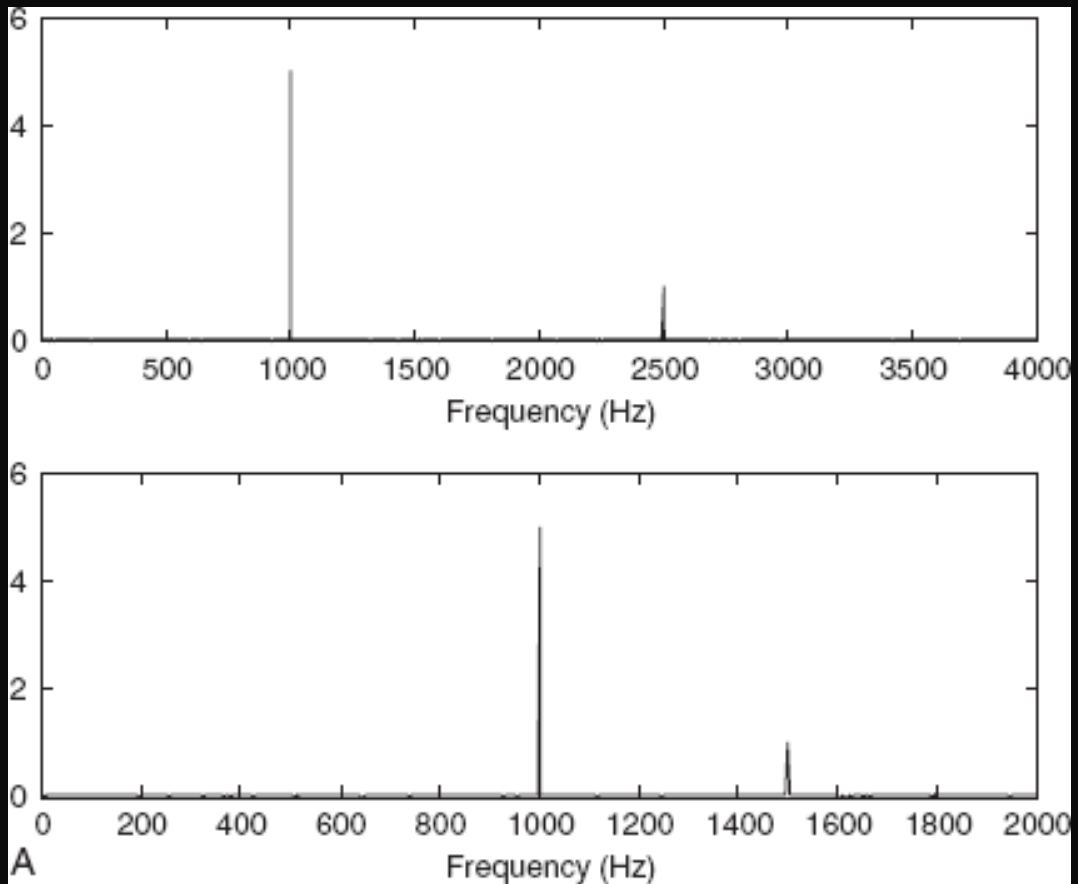
\includegraphics[width=250px,height=140px]{./aliasing_from_downsampling.png}
\caption{Φαινόμαινο αλλοίωσης σήματος μετά την καταγραφή του.}
\end{figure}

Το συμπέρασμα αυτό προέκυψε χρησιμοποιώντας μια μέθοδο που εντάσσεται στην κατηγορία
της επεξεργασίας σημάτων πολλαπλών συχνοτήτων, μεταβάλλοντας την συχνότητα καταγραφής
αφαιρώντας πλήθος δειγμάτων, και συγκρίνοντας τις γραφικές παραστάσεις στα πεδία
συχνοτήτων και χρόνου.
Την απόρριψη του συγκεκριμένου τύπου "θορύβου" στις σύγχρονες συσκευές αναλαμβάνουν
ειδικά φίλτρα που ονομάζονται φίλτρα που ονομάζονται \(\en{F.I.R.}\). Περισσότερα θα αναφερθούν
αργότερα.

\selectlanguage{english}
\url{https://en.wikipedia.org/wiki/Anti-aliasing\_filter}
\selectlanguage{greek}

\chapter{Μείωση αριθμού δειγμάτων}
\label{sec:org61e6d79}
Η τεχνική αυτή εφαρμόζεται σε ψηφιακά σήματα με πολλά δείγματα ανά
χρονικό διάστημα που όμως η τυπική απόκληση προδίδει μια περιοδική
κίνηση που σχετίζεται με ταλάντωση. Τότε είναι εύλογο να χωριστεί το
σήμα σε μικρότερα “κομμάτια”. Αύτο έχει σαν αποτέλεσμα την ταχύτερη
ανάλυση των δεδομένων και την ευελιξία της επιλογής ομάδων σε συνάρτηση
με τον χρόνο ή κάποιο άλλο κριτήριο. Εφαρμόζεται συχνά στην
καθημερινότητά μας, καθώς η συμπίεση αρχείων και τα πρότυπα αρχεία ήχου
και εικόνας συμπεριλαμβάνουν μία ή και περισσότερες διαδικασίες μείωσης
του αριθμού των δειγμάτων.

Στην επεξεργασία ψηφιακών σημάτων οι όροι μείωση αριθμού δειγμάτων,
αποδεκατισμός και συμπίεση μπορεί να έχουν ταυτόσημα νοήματα ή μπορεί να
περιγράφουν την απομείωση συχνοτήτων και απορριψη αριθμού δειγμάτων σε
ένα σύστημα ψηφιακής καταγραφής σημάτων πολλαπλών συχνοτήτων. Αργότερα
θα αναλυθεί η σημασία τέτοιων συστημάτων.

Αποδεκατισμός ενός ψηφιακού σήματος σημαίνει η αποθήκευση τελικώς του
κάθε 10ου δείγματος από το αρχικό καταγεγραμμένο σήμα με συγκεκριμένη
συχνότητα καταγραφής. Αυτό έχει επεκταθεί ορίζοντας τον αποδεκατισμό
κατά έναν παράγοντα που συνήθως είναι σταθερός αριθμός και μπορεί να
λάβει ακέραιες και δεκαδικές τιμές.
Έδω αξίζει να σημειωθεί η ανάγκη να λαμβάνει ο παράγοντας αυτός μια
λογική τιμή, για παράδειγμα ένα ψηφιακό σήμα που έχει διάρκεια πέντε
(5) δευτερόλεπτα και καταγράφηκε από συσκευή που είχε συχνότητα
καταγραφής 20 \(\en{Hertz}\) ένας παράγοντας 101 προφανώς δεν θα άφηνε κανένα
δείγμα στο νέο ψηφιακό σήμα. Επιπρόσθετα το όριο για να αποφύγουμε την
αλλοίωση απαιτεί το τελικό αποτέλεσμα των διαδικασιών είναι τα 10
δείγματα ανά δευτερόλεπτο (10 \(\en{Hz}\)). Επομένως θέτοντας τον παράγοντα
αποδεκατισμού 51 θα παρείχε ένα σήμα που θα ήταν αλλοιωμένο.Όταν η
διαδικασία αυτή εφαρμόζεται σωστά σε μια αλληλουχία δειγμάτων ενός σήματος
ή μιας συνεχής συνάρτησης, παράγεται μια προσομοίωσή του καταγεγραμμένο
με μικρότερη συχνότητα.
Όταν το φίλτρο κατά της αλλοίωσης είναι σχεδιασμένο με πρότυπο \(\en{IIR}\), τα
οποία θα αναλυθούν παρακάτω, η διαδικασία βασίζεται στην ανάδραση της
εξόδου στην είσοδο του φίλτρου πριν την έναρξη του δεύτερου στάδιου. Για
το πρότυπο σχεδιασμού \(\en{FIR}\) είναι εύκολο να υπολογιστεί για κάθε Μ εξόδου.
Ο υπολογισμός που γίνεται από ένα τέτοιο φίλτρο αποδεκατισμού για κάθε
νιοστή έξοδο δείγματος φαίνεται παρακάτω.

\begin{equation}
y[n]=\sum_{k=0}^{K-1}x[nM-k] \cdot h[k],
\end{equation}


Όπου η ακολουθία \(\en{h}\)[•] είναι η απόκριση του κρουστικού παλμού (\(\en{impulse\ response}\))
, και K είναι το μήκος. Η \(\en{x}\)[•] αντιπροσωπεύει το σήμα εισόδου
εξαγόμενο από το φίλτρο με λιγότερα δείγματα.
Σε επεξεργαστές γενικής χρήσης μετά τον υπολογισμό της παραπάνω εξίσωσης
για κάποιον αριθμό \(\en{n}\), ο ευκολότερος τρόπος να υπολογιστεί το \(\en{y[n+1]}\)
είναι η καθυστέρηση της αρχής της ακολουθίας \(\en{x}\)[•] κατά Μ, και να λυθεί
το παραπάνω άθροισμα ξανά. Άν ο παράγοντας Μ=2, η συνάρτηση \(\en{h}\)[•] μπορεί
να αντιπροσωπεύει ενα φίλτρο μισών συχνοτήτων, όπου σχεδόν το μισό πλήθος
των δειγμάτων του αρχικού σήματος θα είναι μηδενικής ισχύος (\(\en{amplitute}\))
και δεν θα συμπεριληφθούν στο προϊόν πολλαπλασιασμού.
Οι \textbf{τιμές} της απόκρισης του παλμού κατά διαστήματα Μ δημιουργούν
υποαληλλουχίες, πλήθους Μ περιπλεγμένες μεταξύ τους.Το παράγογο του
πολλαπλασιασμού είναι η πρόσθεση των προϊόντων από τον πολλαπλασιασμό
κάθε υποαληλλουχίας με το καταγεγραμμένο σήμα \(\en{x}\)[•]. Επιπρόσθετα λόγω
της μειώσης του πλήθους των δειγμάτων στο σήμα κατά Μ, κάθε σήμα που
χρησιμοποιήθηκε στον προηγούμενο υπολογισμό κάποιου Μ προϊόντος δεν θα
επαναλληφθεί σε επόμενο υπολογισμό. Αυτός είναι και ο λόγος που τα φίλτρα
μικρής τάξης Μ \(\en{FIR}\) φιλτράρουν μια από τις αλληλουχίες της εισόδου κάθε
φορά και τα Μ προϊόντα προσθέτονται για να κατασκευαστεί το σήμα εξόδου.
Αυτή η μέθοδος εφαρμόζεται σε συστήματα πολλαπλών επεξεργαστών, όπου ένα
σήμα χωρίζεται σε φάσεις και φιλτράρεται ξεχωριστά από Μ αριθμό φίλτρων
και τελικά προσθέτονται για την δημιουργία του σήματος εξόδου. Τα παραπάνω
φίλτρα ονομάζονται και πολυφασικά.
Για εγκυκλοπεδικούς λόγους αξίζει να σημειωθεί πως είναι πιθανό σε κάθε
φάση του υπολογισμού να αντικαθιστούμε τις τιμές της προηγούμενης φάσης
με μηδενικές τιμές, σε ένα αντίγραφο της αλληλουχίας \(\en{h}\)[•], επεξεργάζοντας
το αρχικό σήμα στην συχνότητα εισόδου (πολλαπλασιάζοντας με 0) και
αποδεκατίζοντας την έξοδο κατά έναν παράγοντα Μ. Η παραπάνω διαδικασία
ονομάστηκε στα αγγλικά \(\en{the\ first\ Noble\ identity}\) και εφαρμόζεται σε
διαφοροποιημένες πολυφασικές μεθόδους.

\selectlanguage{english}
\begin{itemize}
\item \href{https://en.wikipedia.org/wiki/Downsampling\_(signal\_processing)}{wikipedia}
\end{itemize}
\selectlanguage{greek}

\noindent\rule{\textwidth}{0.5pt}

\part{Επεξεργασία σημάτων}
\label{sec:orgfb10a8f}

\chapter{Ορισμός μετα-επεξεργασίας}
\label{sec:orgd060803}
    Η επεξεργασία ενός σήματος θα πρέπει να γίνεται με προσοχή καθώς είναι
εύκολο να καταστραφεί μέρος της πληροφορίας που περιέχεται ή ακόμα και
να εκδοθούν λανθασμένα συμπεράσματα για την συμπεριφορά του συστήματος.
Εδώ χρησιμοποιήθηκε η \textbf{μετα-επεξεργασία} , δηλαδή τα δεδομένα
καταγράφηκαν με σταθερή συχνότητα δειγματοληψίας σε μορφή αρχείου
δεδομένων (\(\en{datasets}\)) .\(\en{tdms}\) μέσω του προγράμματος \(\en{LabView}\).

    Η μέθοδος αυτή δίνει την δυνατότητα στον αναλυτή να επεξεργαστεί τα
δεδομένα στον προσωπικό του υπολογιστή ακόμα και να συνδεθεί σε κάποιον
ισχυρότερο υπολογιστή και να τα διαχειριστεί εξ’ αποστάσεως. Μπορεί όμως
να γίνεται και στην εγκατάσταση αυτοματοποιώντας την διαδικασία
καταγραφής των δεδομένων. Τα συστήματα τηλεπικοινωνιών βασίζονται στην
σωστή κωδικοποίηση από τον πομπό και αποκωδικοποίηση στον δέκτη, οι
διαδικασίες αυτές λαμβάνουν χώρα στις συσκευές που καταγράφουν και
μεταδίδουν το σήμα, όμως επειδή η επεξεργασία της
κωδικοποίησης-αποκωδικοποίησης γίνεται αφού καταγραφεί το σήμα σε κάποια
προσωρινή ή μόνιμη μνήμη και έτσι εντάσσεται στην \textbf{μετα-επεξεργασία}.

\chapter{Εγκατάσταση εργαστηρίου}
\label{sec:orgb208c28}
    Η εγκατάσταση που χρησιμοποιήθηκε για την συλλογή των δεδομένων
αποτελείται από μία αεροσύραγγα την οποία τροφοδοτεί με σταθερή ταχύτητα
αέρα ένας ηλεκτροκινητήρας προσδεδεμένος σε έναν έλικα. Στην μέση της
σήραγγας υπάρχει ένα πλέγμα διάχυσης ώστε η ροή του αέρα να γίνεται όσο
το δυνατόν πιο ομοιόμορφα στην έξοδο όπου βρίσκεται και το αισθητήριο
όργανο για την καταγραφή της ταχύτητας του ανέμου. Παρακάτω φαίνεται μια
εικόνα της εγκατάστασης σε σχηματικό διάγραμμα.

\begin{figure}[htbp]
\centering
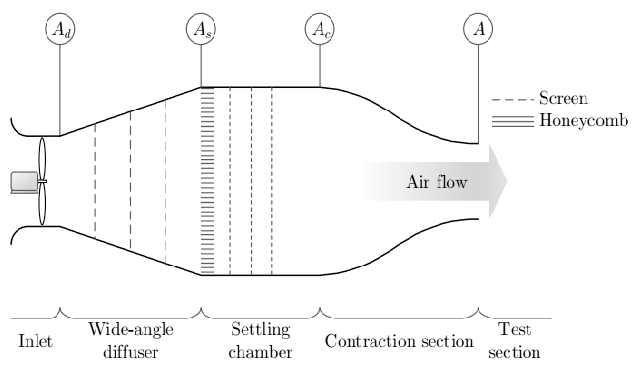
\includegraphics[width=420px,height=250px]{./Wind_Tunnel_setup_lab.png}
\caption{Θάλαμος ομοιόμορφης παροχής ανέμου στο αισθητήριο όργανο όπου τοποθετείται στο σημείο \textbf{Α}. Στο σημείο  \textbf{\(A_{s}\)}, βρίσκεται ένα πλέγμα διάσπασης της ροής που μας επιτρέπει την ομαλή ταχύτητα στο σημείο εξόδου \textbf{A}.}
\end{figure}


    Ένας λόγος που δεν χρησιμοποιήθηκε επεξεργασία σε πραγματικό χρόνο είναι
ότι η εγκατάσταση "που χρησιμοποιήθηκε για την συλλογή των δεδομένων"
κατασκευάστηκε με σκοπό την σύνδεσή του σε κεντρική μονάδα επικοινωνίας
και από εκεί πραγματοποιείται σύνδεση μέσω σειριακής θύρας \(\en{USB}\) με Η/Υ,
όπου και καταγράφεται το σήμα του αισθητήριου οργάνου (\(\en{pitot-tube}\)). Ένας
δεύτερος λόγος ήταν η ανάγκη να δοκιμαστούν διαφορετικές μέθοδοι
αφαίρεσης του θορύβου και προφανώς αυτό θα ήταν πιο δύσκολο εάν έπρεπε
να γίνει σε πραγματικό χρόνο αλλάζοντας τις απαραίτητες παραμέτρους για
την ρύθμιση του φίλτρου. Θα έπρεπε λοιπόν να εγκατασταθεί ανάλογη
συσκευή, όπως ένας μικροεπεξεργαστής, που θα είχε την δυνατότητα για
υψηλές ταχύτητες δειγματοληψίας καθώς η καταγραφή έγινε στα 100 \(\en{kHz}\).
Αυτό θα αύξανε πολύ το κόστος της κατασκευής και θα απαιτούσε
βαθμονόμιση του φίλτρου για να μην προστεθεί περαιτέρω σφάλμα στην
μέτρηση

\noindent\rule{\textwidth}{0.5pt}

\part{Σχεδιασμός Φίλτρων}
\label{sec:org1e8e998}

\chapter{Κατηγορίες}
\label{sec:org5acf0ef}
Λόγω των πολλών εφαρμογών που έχουν και την εκθετική αύξηση της χρήσης
ηλεκτρονικών συσκευών στην καθημερινότητα, οι δυνατότητες επεξεργασίας
ψηφιακών σημάτων αποτελεί πρακτικά απαραίτητη προϋπόθεση. Έτσι η ανάγκη
για την ανάπτυξη διαφόρων τύπων φίλτρων π.χ. το φίλτρο μέσης τρέχουσας
τιμής (\(\en{F.I.R.}\)), το φίλτρο άπειρης κρουστικής απόκρισης (\(\en{I.I.R.}\)) και το μεσιανό
φίλτρο (\(\en{median\ filters}\)). Στην συνέχεια θα αναφερθούμε και στις τρείς αυτές
κατηγορίες αναφέροντας παραδείγματα από τις μεθόδους που χρησιμοποιήθηκαν
στην ανάλυση των δεδομένων από την \textbf{εργαστηριακή εγκατάσταση} ? \ldots{}
Η γενική διαφοροποίηση που γίνεται αρχικά είναι ώς προς το εύρος
συχνοτήτων που επηρεάζουν. Έτσι αν απορρίπτονται οι ύψηλες συχνότητες, το
φίλτρο ονομάζεται διέλευσης χαμηλών συχνοτήτων (\(\en{low-pass\ filter}\))
ενώ το αντίστροφο ονομάζεται φίλτρο διέλευσης υψηλών συχνοτήτων (\(\en{high-pass\ filter}\)).
Άν το φίλτρο επηρεάζειμία περιοχή ή \textbf{φάσμα} συχνοτήτων και
απορρίπτει όσες βρίσκονται πριν και μετά, ονομάζεται φίλτρο απόρριψης
εύρους συχνοτήτων (\(\en{band-stop\ filter}\)).

\chapter{Φίλτρο άπειρης κρουστικής απόκρισης}
\label{sec:org5c63909}
Τα φίλτρα άπειρης κρουστικής απόκρισης στο πεδίο του χρόνου <216>\ldots{}.
Γραμμικότητα και χρονική αμεταβλητότητα \ldots{}. <219>\ldots{}..
κλπ \ldots{}..
\ldots{}.

\section{Παραδείγματα με κώδικα}
\label{sec:org979700c}
\textbf{Εδω να μπει μια επεξηγηση για την κατασκευη και εξαγωγή των παρακατω διαγραμμάτων.}
\selectlanguage{english}
\begin{enumerate}
\item Butterworth
\label{sec:org1ddd574}


\begin{minted}[]{python}
# 4TH ORDER BUTTERWORTH FILTER WITH A GAIN DROP OF 1/sqrt(2) AT 0.4 CYCLES/SAMPLE
bb, ab  = signal.butter (4, 0.8, 'low', analog=False, output='ba')
print ('Coefficients of b = ', bb)
print ('Coefficients of a = ', ab)
wb, hb = signal.freqz(bb, ab)
wb = wb/(2*math.pi)
plt.plot(wb, abs(np.array(hb)))

plt.title('Butterworth filter frequency response')
plt.xlabel('Frequency [cycles/sample]')
plt.ylabel('Amplitute [dB]')
plt.margins(0, 0.1)
plt.grid(which = 'both', axis='both')
plt.savefig('Butterworth Filter Freq Response.png')
\end{minted}

\begin{center}
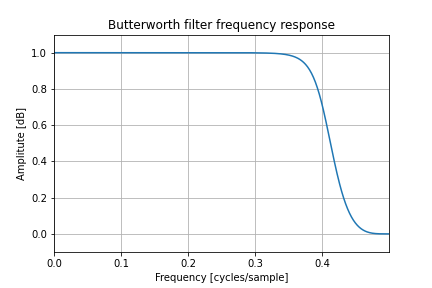
\includegraphics[width=.9\linewidth]{./Butterworth Filter Freq Response.png}
\end{center}

\item Bessel
\label{sec:org5f89dd1}

\begin{minted}[]{python}
# 4TH ORDER BESSEL FILTER WITH A GAIN DROP OF 1/sqrt(2) AT 0.4 CYCLES/SAMPLE

bb, ab = signal.bessel (4, 0.8, 'low', analog=False, output='ba')
print ('Coefficients of b = ', bb)
print ('Coefficients of a = ', ab)
wb, hb = signal.freqz(bb, ab)
wb = wb/(2*math.pi)
plt.plot(wb, abs(np.array(hb)))

plt.title('Bessel filter frequency response')
plt.xlabel('Frequency [cycles/sample]')
plt.ylabel('Amplitute [dB]')
plt.margins(0, 0.1)
plt.grid(which= 'both', axis= 'both')
plt.savefig('Bessel Filter Freq Response.png')
\end{minted}

\begin{center}
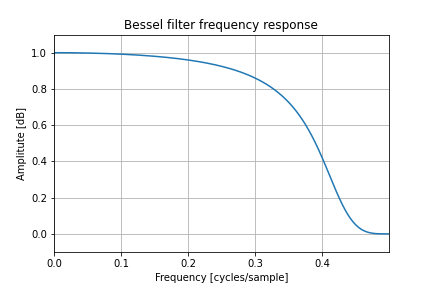
\includegraphics[width=.9\linewidth]{./Bessel Filter Freq Response.png}
\end{center}
\item Chebyshev
\label{sec:org6b08d45}

\begin{minted}[]{python}
#4TH ORDER CHEBYSHEV FILTER TYPE 1 (ONLY IN PASSBAND RIPPLES)
#WITH MAX RIPPLES=2 AND THE GAIN DROP AT 1.5 CYCLES/SAMPLE

bb, ab = signal.cheby1 (4, 2, 0.3, 'low', analog=False, output='ba')
print ('Coefficients of b = ', bb)
print ('Coefficients of a = ', ab)
wb, hb = signal.freqz(bb, ab)
wb = wb/(2*math.pi)
plt.plot(wb, abs(np.array(hb)))

plt.title('Chebyshev filter frequency response')
plt.xlabel('Frequency [cycles/sample]')
plt.ylabel('Amplitute [dB]')
plt.margins(0, 0.1)
plt.grid(which= 'both', axis= 'both')
plt.savefig('Chebyshev Filter Freq Response.png')
\end{minted}

\begin{center}
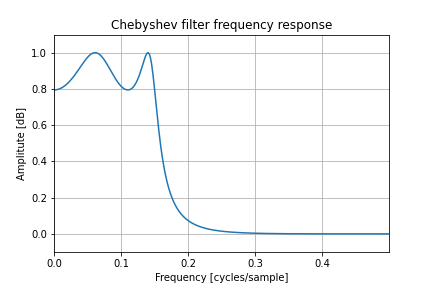
\includegraphics[width=.9\linewidth]{./Chebyshev Filter Freq Response.png}
\end{center}
\item Elliptic
\label{sec:org1fac093}

\begin{minted}[]{python}
# 4TH ORDER ELLIPTIC FILTER WITH MAX RIPPLES =2dB IN PASSBAND,
# MIN ATTENUATION =8dB IN STOP BAND AT 0.25 CYCLES/SAMPLE

bb, ab = signal.ellip (4, 2, 8, 0.5, 'low', analog=False, output='ba')
print ('Coefficients of b = ', bb)
print ('Coefficients of a = ', ab)
wb, hb = signal.freqz(bb, ab)
wb = wb/(2*math.pi)
plt.plot(wb, abs(np.array(hb)))

plt.title('Elliptic filter frequency response')
plt.xlabel('Frequency [cycles/sample]')
plt.ylabel('Amplitute [dB]')
plt.margins(0, 0.1)
plt.grid(which= 'both', axis= 'both')
plt.savefig('Elliptic Filter Freq Response.png')
\end{minted}

\begin{center}
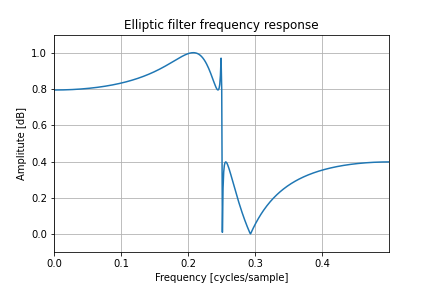
\includegraphics[width=.9\linewidth]{./Elliptic Filter Freq Response.png}
\end{center}

\end{enumerate}
\selectlanguage{greek}
\end{enumerate}
\chapter{Φίλτρο μέσης τρέχουσας τιμής}
\label{sec:org5d17df1}
Η κατηγορία αυτή εξειδικεύεται περαιτέρω, εφαρμόζοντας μια μέθοδο παραθύρων
τα οποία προσφέρουν συγκεκριμένες αποκρίσεις στο πεδίο των συχνοτήτων. Μερικά
παραδείγματα θα παρουσιαστούν παρακάτω, καθώς ήταν μια από τις μεθόδους που
εξετάστηκαν κατά την διάρκεια της ανάλυσης των δεδομένων. Παρείχε αποτελέσματα
που ενέτασαν στην έξοδό του ενίσχυση του σήματος σε χαμηλές συχνότητες. Αύτο
ήταν αποτέλεσμα του τρόπου με τον οποίο ορίζεται ο συγκεκριμένος τύπος, καθώς
φαίνεται να μην συνιστάται όταν ο όγκος δεδομένων έχουν μεγάλο πλήθος. Ο λόγος
είναι ότι πρέπει να οριστεί ένα πολυώνυμο με το οποίο κάθε συντελεστής ταυτίζεται
με κάθε ένα από τα σημεία του δείγματος. Έτσι σε μεγάλα σετ δεδομένων απαιτείται
πρακτικά μεγάλος όγκος αριθμητικών υπολογισμών που καθυστερεί την έκβαση των
αποτελεσμάτων σε μη αποδεκτό βαθμό.
\section{Κατηγορίες παραθύρων φίλτρων πεπερασμένης κρουστικής απόκρισης}
\label{sec:org345bd43}

\begin{enumerate}
\item Συχνοί τύποι παραθύρων
\label{sec:orgacd7cb8}
\begin{itemize}
\item Βασικές κατηγορίες φίλτων:
\begin{itemize}
\item \(\en{Rectangle}\)

\item \(\en{Barlett}\)

\item \(\en{Hanning}\)

\item \(\en{Hamming}\)
\end{itemize}
\end{itemize}

\item Μέθοδος \(\en{Kaiser}\)
\label{sec:orgeb536c2}

\item Βέλτιστες προσομοιώσεις φίλτρων
\label{sec:orgb45ae2a}

\selectlanguage{english}
\begin{itemize}
\item Here is a deep analysis for the appropriate implementation of the FIR filters in respect to \emph{M value???}
\end{itemize}
\selectlanguage{greek}

\noindent\rule{\textwidth}{0.5pt}
\end{enumerate}
\part{Βιβλιογραφία}
\label{sec:orgf0c7c7d}
\selectlanguage{english}

\noindent
Edmund Lai (2003). \emph{6 - Finite impulse response filter design}, Newnes.

\noindent
Ibrahim Abdulhadi Sulaiman and Hussain Mohammad Hassan and Mohammad Danish and Munendra Singh and P.K. Singh and Manisha Rajoriya (2022). \emph{Design, comparison and analysis of low pass FIR filter using window techniques method}, Materials Today: Proceedings.

\noindent
Koichi Ichige and Naohisa Otsuka and Rokuya Ishii (1997). \emph{An automatic design procedure of IIR digital filters from an analog low-pass filter}, Signal Processing.

\noindent
McClellan, J.H. and Schafer, R.W. and Yoder, M.A. (2003). \emph{Signal Processing First}, Pearson/Prentice Hall.

\noindent
N. Agrawal and A. Kumar and Varun Bajaj and G.K. Singh (2021). \emph{Design of digital IIR filter: A research survey}, Applied Acoustics.

\noindent
Oppenheim, Alan V. and Schafer, Ronald W. and Buck, John R. (1999). \emph{Discrete-Time Signal Processing}, Prentice-hall Englewood Cliffs.

\noindent
Ryan B. Spelay and Kofi Freeman Adane and R. Sean Sanders and Robert J. Sumner and Randall G. Gillies (2015). \emph{The effect of low Reynolds number flows on pitot tube measurements}, Flow Measurement and Instrumentation.

\noindent
Yong Moon Choi and Yoshiya Terao and Noboru Kurihara and Aya Iwai and Tatsuya Funaki and Woong Kang and Doan Trang Nguyen (2021). \emph{Revisit the Pitot static tubes in the standards}, Flow Measurement and Instrumentation.
\end{document}